%\externaldocument{appendix_tor_model}
\chapter{Structural Changes in Doped and Excited Conjugated Polymers}

\section{Introduction}

Conjugated polymers are promising materials for use in a range of applications such as light-emitting diodes, solar cells, battery materials, transistors, and actuators for artificial muscles \cite{Swager2017}. These applications rely on the material being doped and/or excited, where the resulting electronic conductivity and more specifically carrier mobility is governed by polymer chain structure \cite{Noriega2013a, Noriega2013}. Although chain structure dictates carrier mobility, relatively little is known about the structure of doped or excited chains, especially at larger length scales ($\geq 5 \ nm$). At smaller length scales ($< 5 \ nm$) polarons and excitons are known to cause local structural distortions via electron-vibrational and electron-torsional coupling \cite{Tapping2014, Zhou2015, Yu2012, Busby2011}, but the collective impact on chain structure has not been quantified. Structural knowledge is fundamental to improving carrier mobility and other electronic properties in conjugated polymer materials \cite{Beaujuge2011, Kuei2017}.

In general, conjugated polymers at room temperature exhibit a mixture of semicrystalline and amorphous domains \cite{Shen2016}. Emerging research have shown that connectivity between semicrystalline or disordered aggregate domains is critical, and surprisingly an increase in crystallinity does not equate to an increase in bulk carrier mobility \cite{Son2016, Noriega2013}. Instead, it is the specific material's ability to remain electronically connected while experiencing an inevitable amount of disorder that governs its conductivity \cite{Noriega2013}, as opposed to the intrinsic conductivity of a polymer chain. Both Son et al. and Noriega et al. provide schematics, on the domain level, to help visualize these concepts \cite{Son2016, Noriega2013}.

The ability of conjugated polymer materials to remain electronically connected depends on the structure of the amorphous chains that physically connect the semicrystalline or disordered aggregate domains \cite{Noriega2013}. Carrier mobility in amorphous regions is particularly sensitive to individual chain structure because chains regularly adopt non-planar conformations\footnote[2]{Although conformation and configuration are used somewhat interchangeably to describe polymer structure, for the purposes of this article, a conformation refers to the structure of an entire chain, whereas a configuration refers to local structure within a chain (e.g. a torsional configuration).} \cite{Noriega2013a}. If a chain torsion angle is in a sufficiently non-planar configuration\footnotemark[2], the conjugation pathway along the chain is disrupted, due to less p-orbital overlap, thus creating an energy barrier to transport that is insurmountable by carriers at room temperature. Disrupted conjugation essentially acts as a dead end \cite{Son2016}, similar to a kink in a garden hose blocking the flow of water. Aromatic conjugated polymers (e.g. polythiophene (PT), poly(3-hexylthiophene) (P3HT), polypyrrole (PPy), and poly(p-phenylene vinylene) (PPV)) are representative of chains that adopt non-planar torsional configurations in their ground state (undoped and unexcited) and will be the focus of this study \cite{Dubay2012, Fonner2010, Kofranek1992, Mao1993}. Furthermore, we place emphasis on polythiophenes because both PT and P3HT have recently been utilized in high mobility disordered polymers \cite{Son2016, Zhang2010}.

\begin{figure*}[hbt!]
  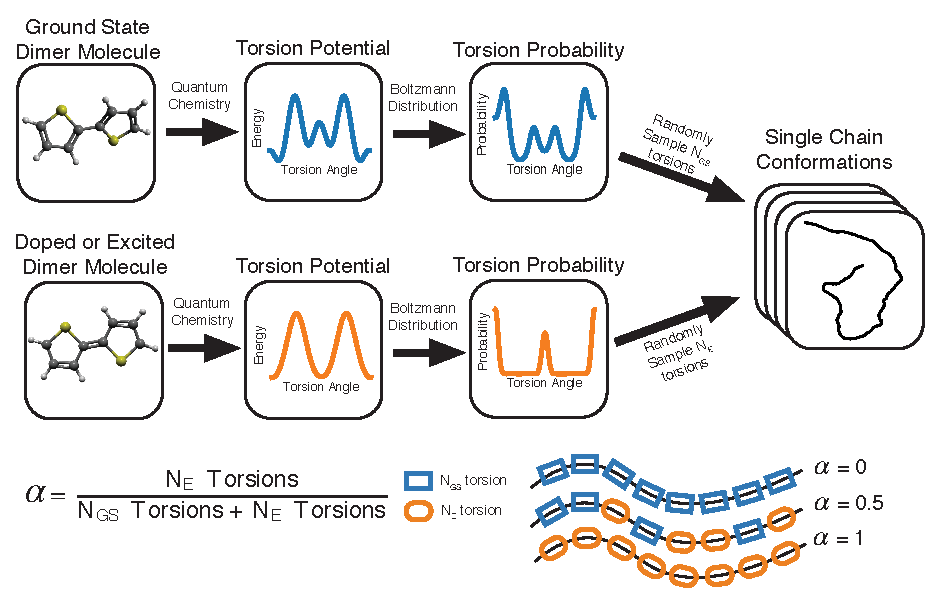
\includegraphics{figures/chap2/methods_diagram.pdf}
  \caption[Algorithm of the Torsion Potential Model]{The torsion potential model algorithm for generating ensembles of single chain conformations. The variable $\alpha$ represents the fraction of doped or excited torsion angles along a chain.}
  \label{fig:TPM}
\end{figure*}

\clearpage

A torsion-based approach to modeling doped and excited chains utilizes previous methods, and is physically motivated by the torsional nature of the doping and excitation process in aromatic conjugated polymers. Although amorphous polymers possess many structural degrees of freedom, and statistical averages are necessary to describe the ensemble of conformations, the problem of modeling individual chains can be greatly simplified by allowing only the torsional degrees of freedom to fluctuate \cite{Flory1989}. Taking this a step further, if neighboring torsion angles can be considered independent, individual chains are reduced to a set of uncorrelated torsion angles. This later assumption has been shown to be valid for semiflexible polymers such as PT and P3HT \cite{Westenhoff2006, Zhang2014}. As a result, chain models based on torsion potentials have been developed for aromatic conjugated polymers (e.g. PT and PPV) \cite{Zhang2014, Claudio2001}, however, the effect of doping or excitation has not been considered.

In this article we determine the impact of torsional rearrangements, due to doping or excitation, on amorphous chain conformations and properties. Additionally, it is evident that these chains undergo fast and substantial nuclear relaxation upon doping or excitation \cite{Zhou2015, Busby2011}, hence our objective is to study steady-state chain conformations and properties as a function of the doping or excitation level. A better understanding of these structural changes will provide insight for a variety of on-going and future strategies directed at tuning electronic conductivity of conjugated polymers.

\section{Model}

We developed a stochastic torsion potential model for generating chain conformations at various levels of doping and excitation, outlined in Fig.~\ref{fig:TPM}. A brief description of the model is provided here with more details in the Methods and Appendix A. First, we calculate dimer ground, doped (cation), and excited (first triplet) state torsion potentials using quantum chemistry. Next, room temperature Boltzmann distributions are computed from associated torsion potentials. Finally, chain conformations are generated by randomly sampling the Boltzmann distributions based on the fraction of doped and excited torsion angles ($\alpha$). After sampling an ensemble of chain conformations at each $\alpha$ value average chain properties such as persistence length, end-to-end distance, and planarity (S order parameter) can be calculated.

\section{Results and Discussion}
\subsection{Torsion Potentials}

\begin{figure*}[hbt!]
    \centering
    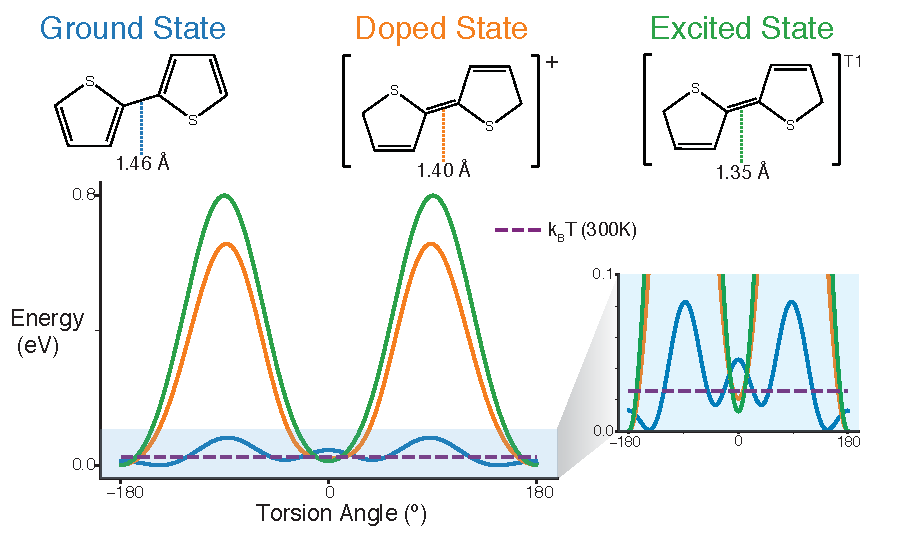
\includegraphics{figures/chap2/tor_compare.pdf}
    \caption[Comparison of the Ground, Doped, and Excited-state Torsion Potentials]{A comparison of torsion potentials, bridge bond lengths, and structures of the ground, doped (cation), and excited-state (triplet) thiophene dimer molecules. The doped and excited states are represented as quinoidal structures.}
    \label{fig:comp_tor}
\end{figure*}

When comparing the PT torsion potentials from Fig.~\ref{fig:comp_tor}, the doped and excited potentials are qualitatively similar, yet very different from the ground state. Throughout the work presented here, the doped state refers to calculations performed on a cation dimer, and the excited state refers to dimer calculations performed on the lowest energy excited state (i.e. the first triplet T1). While a direct photoexcitation to the lowest energy state (T1) is spin-forbidden it is accessed via intersystem crossing \cite{Beljonne2001, Banerji2011, Kolle2016}, and hence a good representation for steady-state behavior. In both the doped and excited potentials the number of minima and maxima are reduced, the location of the minima are shifted to planar configurations, and the relative barriers between extrema are much larger. A similar trend can seen for PPy in Fig. \ref{fig:ppy_tor}. The overall shape of the calculated torsion potentials is not sensitive to the level of quantum chemistry theory or basis set used (see Fig. \ref{fig:gs_theory}), which suggests that the underlying physics are well captured. Nevertheless, we emphasize that the level of theory and basis set are important for capturing quantitative energy differences between configurations, especially for the cis (0\textdegree \ torsion angle) and trans (180\textdegree \ torsion angle) configurations in the doped and excited state.

The torsional differences between the doped and excited states and the ground state are due to an electronic structure rearrangement. Previous efforts have reported a transition from ground-state aromatic structure to quinoidal structure upon doping or excitation for a variety of conjugated polymers (aromatic and quinoidal PT structures are displayed at the top of Fig.~\ref{fig:comp_tor}) \cite{Roth2013_ch5, Burrezo2017, Wells2008, Aime1989, Banerji2011, Roseli2017, Busby2011, Yu2014, Fonner2010, Baitoul2000, Bradley1989}. Our results for PT and PPy (Appendix \ref{sec:ppy}) support this conclusion. Doped and excited bridge C-C bond lengths were shorter as compared to that of the ground state (Fig. \ref{fig:comp_tor}), signifying double bond character in the doped and excited states. Additionally, the doped and excited-state torsion potentials resemble that of ethylene, which has an ideal bridge C=C double bond \cite{Shao2003}. Pronounced resonance (electron delocalization) is observed in both the doped and excited structures, such that the bridge C-C bonding character falls somewhere between a single and double bond. The excited state exhibits more double bond character, based on the bridge bond length, which results in a steeper torsion potential as compared to that of the doped state.

A point of contention when determining polymer torsion potentials is the validity of a dimer to accurately represent the torsion potential of the larger chain. Indeed, earlier work on PT and P3HT suggests that longer chains are necessary for determining the torsion potential \cite{Darling2009}. However, DuBay et. al. attributed the chain size effects to inadequate basis set size and relaxation procedure. Furthermore, DuBay et. al. demonstrated that dimers can accurately represent conjugated polymer torsion potentials when a sufficient level of theory, basis set, and relaxation procedure are used \cite{Dubay2012}. Our results, which examined ground-state (undoped and unexcited) chains up to 8 monomers, agree with DuBay et. al. in that chain length does not meaningfully impact the torsion potential of ground-state PT. While this conclusion does not hold a priori for doped or excited torsion potentials due to the additional complications of charge and spin localization, we nevertheless find that the doped dimer suitably characterizes the torsion potential of the larger doped chain. Appendix \ref{sec:pt_tp} contains data and additional insight on the impact of the chain length on torsion potentials.

\subsection{Persistence Length}

\begin{figure*}[hbt!]
    \centering
    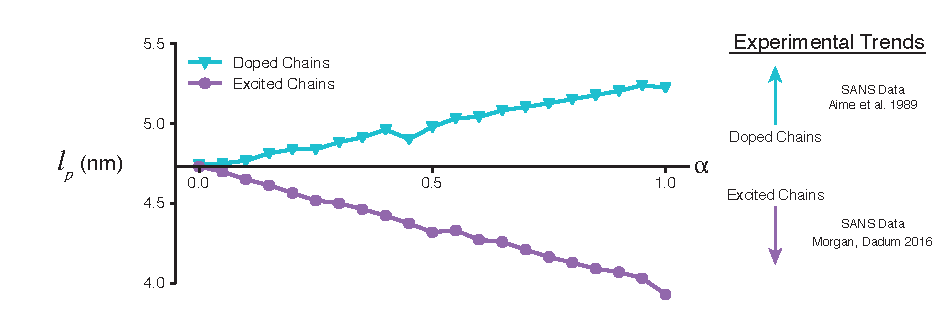
\includegraphics{figures/chap2/persist_len.pdf}
    \caption[Persistence Length Trends for Doped and Excited Chains]{(Left) Calculated persistence lengths ($l_p$) as a function of doping and excitation ($\alpha$). (Right) Experimental persistence length trends for doped and excited chains.}
    \label{fig:lp}
\end{figure*}

The trend in persistence length as a function of $\alpha$ (Fig.~\ref{fig:lp}) highlights an important difference between doped and excited chains. Remarkably, the persistence length and the end-to-end distance of excited chains decrease with increasing $\alpha$. We initially anticipated excited chains to be more linear as a result of the excited-state torsion potential. Indeed, the persistence length and end-to-end distance of doped chains increase with increasing $\alpha$. In both types of chains the end-to-end distance can be related to the persistence length by the worm-like chain (WLC) model (Eq.~\ref{eq:wlc_msqr}).

Comparing the calculated persistence length with experimental values reflects well on the obtained torsion potential model. The calculated ground-state PT persistence length of 4.7 nm, is in good agreement with a recently obtained experimental value of $\sim$ 3 nm for P3HT \cite{Mcculloch2013} and a previous measurement of 5.5 nm for PT \cite{Aime1989}. Moreover, McCulloch et al. observed the trend of decreasing persistence length with increasing side chain length, which indicates that PT should exhibit a persistence length longer than $\sim$ 3 nm. In addition, the persistence length trend calculated for both doped and excited chains qualitatively agree with experimental observations.

\begin{figure*}[hbt!]
    \centering
    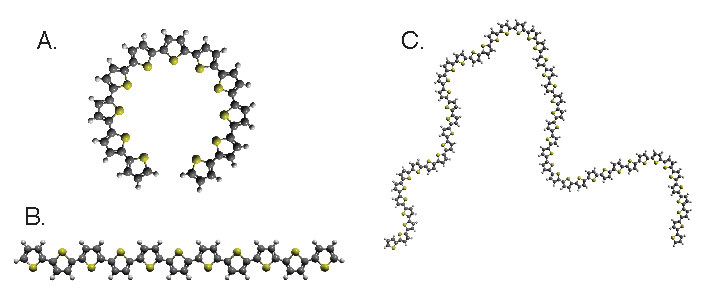
\includegraphics{figures/chap2/planar_chains.pdf}
    \caption[Idealized Cis, Trans, and Mixed Chain Conformations]{(A) Circular all cis chain (B) Linear all trans chain (C) A random 1:1 mixture of cis and trans torsion angles. All conformations are completely planar.}
    \label{fig:ideal}
\end{figure*}

The fraction of cis torsion angles in doped or excited PT chains dictates its persistence length and end-to-end distance. Figure \ref{fig:ideal} demonstrates the impact of cis torsion angles for an idealized case where $\alpha$ = 1 and the torsion angle distribution is reduced to the two minima: 0\textdegree \ (cis) and 180\textdegree \ (trans). Figure \ref{fig:ideal}A and \ref{fig:ideal}B depict the circular cis chain and the linear trans chain respectively. The chain in Fig.~\ref{fig:ideal}C is a random 1:1 mix of cis and trans torsion angles, and clearly illustrates that a chain conformation can be completely planar yet highly non-linear. While the idealized case is an exaggeration of the real doped and excited chains, the histograms of the sampled torsion angles (Fig. \ref{fig:a_0_hist}-\ref{fig:a_1_hist}) demonstrate that the primary difference between the doped and excited chains is the larger fraction of cis or close to cis torsion angles in the excited chains. This can be correlated to the smaller cis-trans energy gap in the excited torsion potential. The larger fraction of cis torsion angles in the excited chains cause them to become more non-linear than the doped chains, explaining the opposing trends in persistence length and end-to-end distance.

A small-angle neutron scattering (SANS) study of PT in solution also observed an increase in persistence length upon doping (Fig. \ref{fig:lp}) \cite{Aime1989}. An undoped PT persistence length of 5.5 nm was reported, in quantitative agreement with our calculated value of 4.7 nm. Aime et al. suggested that highly doped chains were rod-like, and attributed much of change in the persistence length to the ``intrinsic rigidity'' associated with a quinoidal electronic structure. The magnitude of the persistence length increase was considerably larger than the results reported here, but torsional effects may only be partially responsible for the increase in persistence length. More importantly, the rod-like interpretation of the scattering results depends strongly on the scaling of the scattering vector (q), which was found to be $\sim$ q$^{-1}$. Rod-like chains do scale as q$^{-1}$ \cite{Pedersen1997}, but a semiflexible 2D WLC can scale as $\sim$ q$^{-4/3}$ \cite{Cifra2008}. The 2D WLC was not considered at the time, and the resolution of the scattering results may have been insufficient to differentiate between the two. Our results demonstrate the importance of considering chain planarity when interpreting scattering results of doped or excited conjugated polymers.

Another SANS study reported that upon excitation, P3HT chains decrease in length, in alignment with our findings (Fig. \ref{fig:lp}), although the reduction in persistence length reported ($\sim$ 3 nm) slightly exceeds our predictions from torsional effects alone ($\sim$ 1 nm at $\alpha$ = 1) \cite{Morgan2016}. We speculate that other effects such as polymer-solvent interactions may contribute to the overall reduction in length. Additionally, we note that the reduction in chain length from beam damage was not completely clarified. Moreover, Morgan and Dadmun rejected polaron localization and chain planarization as it was assumed that these effects lead to more linear or longer chains, however as shown in this work, chain planarization does not necessarily lead to linear chains.

\subsection{Planarity}

\begin{figure*}
    \centering
    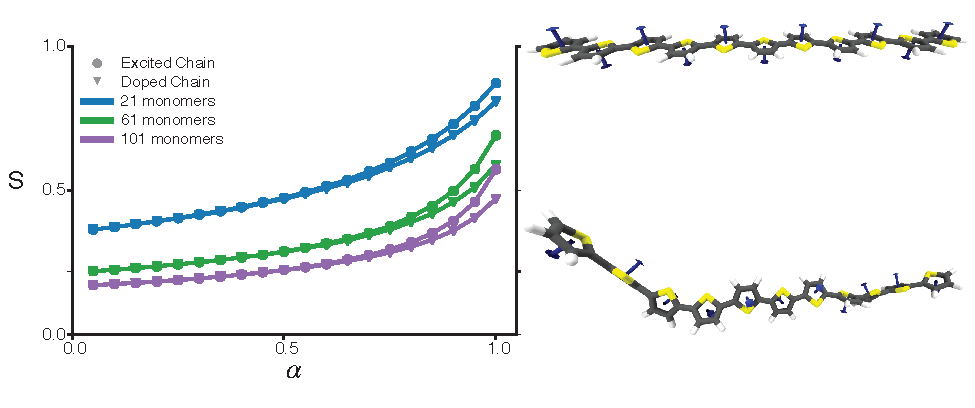
\includegraphics{figures/chap2/S.pdf}
    \caption[Doped and Excited Chain Planarity]{(Left) Chain planarity (S) as a function of doping and excitation ($\alpha$). When S = 0 all thiophene rings have equal probability of facing any direction, whereas when S = 1 the chain is completely planar. (Right) Examples of S = 1 and S $\sim$ 0.2}
    \label{fig:s_order}
\end{figure*}

Figure \ref{fig:s_order} shows the evolution of the order parameter S, which reduces planarity to a single scalar value with a clear physical interpretation. For instance, S = 1 represents a completely planar chain, whereas S = 0 represents an isotropic chain where rings exhibit equal probability of facing any direction. For comparison, typical ordered liquid crystals exhibit S values ranging from 0.3 - 0.8 \cite{Colfen2008}. S does not depend on the ordering of the torsion angles, which renders a more complicated polaron grouping unnecessary for determining S. As seen in Fig. \ref{fig:s_order}, the parameter S monotonically increases with increasing $\alpha$ as expected based on the planar nature of the doped and excited torsion potentials. Although S was calculated for PT we expect the trend to be similar among other aromatic conjugated polymers because the electronic structure rearrangement that fundamentally determines the torsion potential of the doped and excited state is the same. Additionally, S depends on the length of the chain considered. Chain lengths were selected by experimental recommendations for optimum conductivity \cite{Noriega2013}. However, if longer chains are of interest the S values reported here could be viewed as the planarity of a segment along the chain as no chain end effects were considered.

We expect a large increase in S to be associated with an increase in carrier mobility. Carrier mobility in conjugated polymers relies on a continuous conjugation pathway along the polymer backbone \cite{Shin2010}. As mentioned, the conjugation pathway can be disrupted if the rings along the chain are sufficiently non-planar. As a result, a conjugation length can be defined. The order parameter S is intimately related to the conjugation length as both are a measure of planarity, however S is a global measure whereas the conjugation length represents a local feature. Conjugation length is not reported here because it requires explicit treatment of polarons and their interactions to determine the proper ordering/grouping of doped or excited torsion angles along the chain for non-integer values of $\alpha$. We note that ordering does not impact the calculation of S due to the use of the globally defined director. Furthermore, the conjugation length is also dependent on the torsion angle at which conjugation is substantially disrupted (i.e. when the energy barrier to carrier transport is well above thermal fluctuations). Previously, Bredas et al. suggested that torsional configurations which deviate more than 30-40\textdegree \ from planar disrupt electronic properties in aromatic conjugated polymers such as PT and PPy \cite{Bredas1985}. Regardless of the ability to determine the conjugation length, the order parameter S provides evidence that carrier mobility increases with increasing doping or excitation due to torsional rearrangements.

\subsection{Material Design Strategies}

Our results offer a microscopic explanation for the increase of electronic conductivity due to sequential doping, which preferentially dopes amorphous domains in conjugated polymer materials \cite{Chew2017, Jacobs2016}. Compared to other techniques sequential doping improves conductivity, and this has been attributed to an increase in the conjugation length of amorphous chains \cite{Chew2017}. We find that planarity (a measure of conjugation length) increases with doping because of electronic structure and torsional rearrangements. In sum, amorphous chain planarization leads to an increase in carrier mobility and ultimately an improvement of the material's electronic conductivity.

Another method intended to improve electronic conductivity recommends an ultraviolet (UV) treatment to order conjugated polymers in solution before film synthesis \cite{Chang2014}. Organic field-effect transistors made with P3HT films that were pretreated with UV irradiation ($\sim$ 5 mins) exhibited higher carrier mobility compared to those not pretreated. The improvement in mobility was attributed to ``increased molecular order,'' and it was postulated that intrachain planarization induced by excitation caused more interchain $\pi-\pi$ stacking interactions eventually leading to aggregates in solution. These aggregates persisted in the resulting films \cite{Chang2014}, and presumably more uninterrupted conjugation pathways were present. Although unknowns persist about $\pi-\pi$ stacking and polymer-solvent interactions, it is encouraging that device level results agree with the fundamental premise that excitation causes chains to become more planar and that this knowledge can be leveraged to improve materials performance.

Finally, we comment on side chain engineering as a design strategy. Many aromatic conjugated polymers are decorated with side chains, for example P3HT has a PT backbone with a hexyl side chain. Son et al. synthesized P3HT and PT random copolymers to investigate how the ratio impacted carrier mobility. It was the found that introducing more PT reduced crystallinity, increased out-of-plane $\pi-\pi$ stacking, and improved mobility \cite{Son2016}. For our torsion potential model we assume that chains are able reach a thermodynamically favorable conformation, however in certain circumstances bulky side chains may limit backbone torsional rearrangement upon doping or excitation. Thus, lowering side chain density along the polymer backbone may provide a useful strategy to increase the likelihood that a doped or excited backbone torsion angle assumes a planar configuration. A potential exception to this analysis would include bulky side chains that promote planarity in ground-state chains \cite{Raithel2018}.

\section{Conclusion}

The structural properties of amorphous conjugated polymers change as a function of doping and excitation. Initially, aromatic chains undergo a localized electronic structure rearrangement where the bonding pattern is transformed from aromatic to quinoidal. Consequently, the bridge double bond character present in the quinoidal structure drives torsional rearrangement. This description is supported by the reduction in bridge bond lengths as well as the preference for planar configurations in the associated doped and excited-state torsion potentials. To connect electronic structure changes with doped and excited polymer structure we developed a torsion potential model. Our model reproduced experimental persistence lengths for ground-state polythiophene, and the experimental trends in persistence length for doped and excited chains. Chain planarity, which is an important structural property for carrier mobility, monotonically increases with the level of doping or excitation. Notably, our results demonstrated that planar polythiophene conformations can be highly non-linear due to cis torsion configurations. We find that the fraction of cis torsion angles largely dictates the persistence length and end-to-end distance of both doped and excited chains. Excited chains contain a larger fraction of cis torsion angles as compared to doped chains which explains how the trends in persistence length diverge, whereas the trends in planarity are similar. Furthermore, amorphous chain planarization induced by doping and excitation corresponds to enhanced conjugation and ultimately an increase in carrier mobility and electronic conductivity. While more research is needed to adequately characterize doped and excited amorphous chains, the structural insights reported here can be used to interpret characterization data and to advance design strategies aimed at tuning electronic properties in conjugated polymers.

\section{Methods}

\subsection{Torsion Potential Model} The overall torsion potential model methodology has been described by others \cite{Zhang2014, Claudio2001}, but due to our alterations and inclusion of doping and excitation a description is included. A schematic of the model is displayed in Fig.~\ref{fig:TPM}. To start, torsion potentials ($V(\phi)$) for the ground, doped, and excited states were calculated using quantum chemistry. Torsion potentials were fitted using the Ryckaert-Bellemans function (Eq.~\ref{eq:RB}). Details of the fitting procedure and data can be found in Appendix~\ref{sec:TPF}. Each torsion potential was used to generate a room temperature (300 K) Boltzmann probability distribution (Eq.~\ref{eq:Boltz}, where $\beta = 1/k_BT$) for the full range of torsion angles (-180\textdegree \ to 180\textdegree \ with a mesh of 0.1 degrees). The Boltzmann probabilities ($p(\phi)$) were then summed to give cumulative probabilities. Cumulative probabilities (ranging from 0-1) provide a unique torsion angle ($\phi$) mapping that enabled torsion angles to be selected by generating random numbers between 0 and 1. As a result, chain conformations were defined by generating a set of random numbers that correspond to a set of torsion angles. Doping and excitations were introduced by randomly placing doped or excited torsion angles along the ground-state chain. Doped or excited torsion angles were drawn from their respective cumulative probabilities using random numbers similar to the ground state procedure. The variable $\alpha$, which represents the level of doping or excitation, is obtained as the fraction of doped or excited torsion angles. Unless otherwise noted all ensembles at different values of $\alpha$ were sampled with 50,000 conformations.

\begin{equation}
\label{eq:RB}
V(\phi) = \sum_{n=0}^{5} c_n \cos^n(\phi)
\end{equation}

\begin{equation}
\label{eq:Boltz}
p(\phi) = \frac{e^{-\beta V(\phi)}}{\int_{-\pi}^{\pi} d\phi' \ e^{-\beta V(\phi')}}
\end{equation}

The adopted torsion potential model assumes that nearest neighbor torsion angles are independent, and that the torsion potential alone governs single chain conformations. Self-avoidance was not explicitly enforced in our model. We assumed all ground-state chains to be in equilibrium and doped and excited chains in steady-state, signifying that a chain can reach a thermodynamically favorable conformation (i.e. no kinetic limitations). Because we were primarily concerned with equilibrium or steady-state structural properties, we did not consider the torsional dynamics associated with doping or excitation. Doped and excited steady-states require that the number of doped or excited torsion angles remain constant. The steady-state approximation is motivated by recent findings that torsional relaxation upon excitation occurs very rapidly, whereas the torsional relaxation of the reverse process occurs slowly \cite{Busby2011, Yu2016}. Further explanation of the model and its implementation (i.e. the code used) are available in Appendix~\ref{sec:TPM}.

\subsection{Chain Properties}

\begin{figure}
    \centering
    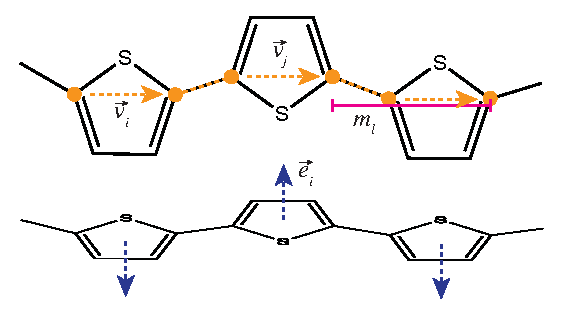
\includegraphics{figures/chap2/bond_vectors.pdf}
    \caption[Backbone Vector, Average Monomer Length, and Ring Normal Vector for PT]{(Top) Backbone vectors ($\Vec{\nu}$) and average monomer length ($m_l$) for PT. (Bottom) Thiophene ring normal vector ($\Vec{e}$)}
    \label{fig:pt_vecs}
\end{figure}

To characterize polymer chain length, we used the persistence length and the root-mean-square end-to-end vector $\sqrt{\big \langle R^2 \big \rangle}$ or simply end-to-end distance. In the torsion potential model end-to-end distance was determined by the scalar displacement from the first carbon atom in the chain to the last carbon atom in the chain. Persistence length ($l_p$) was calculated using the tangent-tangent correlation function (Eq.~\ref{eq:lp}), a relationship that can be derived from the worm-like chain (WLC) model, where $\vec{\nu}_i$ represents the backbone vector i and its correlation with $\vec{\nu}_{i+n}$ the backbone vector $i+n$. Angle brackets $\big \langle \big \rangle$ represent ensemble averages. The contour length (L) of a chain was defined as length of a trans chain (all trans torsion angles, shown in Fig. \ref{fig:ideal}B), and is approximately the monomer number (n) times the average monomer length ($m_l$), $L \approx m_ln$. Backbone vectors, normal vectors, and average monomer length specific to PT are shown in Fig. \ref{fig:pt_vecs}.

\begin{equation}
\Big \langle \large \Vec{\nu_i} \cdot \Vec{\nu_{i+n}} \Big \rangle = \exp{\bigg(-\frac{L}{\chi l_p}\bigg)}
\label{eq:lp}
\end{equation}

The scaling factor $\chi$ in Eq.~\ref{eq:lp} is equal to 1 for a 3-dimensional (3D) WLC and is equal to 2 for a 2-dimensional (2D) WLC \cite{Meyer2016}. By comparing the $\sqrt{\big \langle R^2 \big \rangle}$ for the 3D-WLC, the 2D-WLC, and the torsion potential model (Fig. \ref{fig:gs_wlc}, \ref{fig:d_wlc}, \ref{fig:e_wlc}) we find that for the torsion potential model $\chi$ lies between 1 and 2 in all cases. As a result, $\chi$ was fit for all $\alpha$ values and the fit $\chi$ values were used to determine the persistence length. More details on $\chi$ and persistence length calculations are provided in Appendix~\ref{sec:lp}.

Planarity was also considered in the description and analyses of chain structure. For our purposes, planarity is defined by the orientational order parameter S (Eq.~\ref{eq:S}) \cite{Allen2017}, which is used to quantify molecular orientation in liquid crystals. The variable $\theta$ represents the angle between a thiophene ring's unit normal vector ($\hat{e}$) (Fig.~\ref{fig:pt_vecs}) and the director. The director for a chain is a unit vector that represents the most common direction of ($\hat{e}$), something akin to the average direction of the rings along the chain. See Appendix~\ref{sec:planarity} for details on how S and the director were computed using the orientational order tensor (Q).

\begin{equation}
\label{eq:S}
S = \frac{1}{2} \ \Big \langle \large 3\cos^2\theta - 1 \Big \rangle
\end{equation}

\subsection{Quantum Chemistry Calculations}
Quantum chemistry calculations were used to generate dimer torsion potentials and other structural information. All calculations were performed using QChem software \cite{Shao2015}, Unless otherwise noted, calculations were done in vacuum and the level of theory utilized was the hybrid functional $\omega$B97M-V with basis sets def2-QZVPPD and def2-TZVPPD for ground state and doped/excited states respectively \cite{Mardirossian2016, Weigend2005}. Hybrid density functional theory (DFT) was chosen over second-order M\o ller-Plesset theory (MP2) because of spin contamination issues \cite{Salzner2014}, and basis set sensitivity. Additionally, excited state (T1) calculations were carried out using unrestricted open shell DFT (UO), as both UO and restricted open shell (RO) DFT reproduce experimental results better than time-dependent DFT (TDDFT) for conjugated molecules \cite{Hait2016}. Further discussion and comparison of T1 RO-DFT, UO-DFT, and TDDFT calculations can be found in Table \ref{tab:ex_ct_gap}. The general procedure for all torsion potentials was to do an initial geometry optimization of the dimer, then rotate the central or bridge torsion angle between rings to the angle of interest, and finally run a constrained optimization with the C-C-C-C torsion angle of interest fixed. The last two steps were performed over the range of unique torsion angles.

All doped and excited state calculations were carried out using unrestricted open shell (UO) DFT. Both UO and restricted open shell (RO) DFT reproduce experimental results better than TDDFT for excited conjugated molecules \cite{Hait2016}. A comparison of T1 RO-DFT, UO-DFT, and TDDFT calculations can be found in Table \ref{tab:ex_ct_gap}. It is important to note that RO-DFT or UO-DFT calculations are only reliable for clearly defined HOMO to LUMO transitions, which encompassed all of our T1 torsional configurations with energies relevant for room temperature sampling. However in PT, the nature of the transition at torsion angles around -90\textdegree \ and 90\textdegree \ is affected by other energy levels. As a result, torsion angles around -90\textdegree \ and 90\textdegree \ may benefit from refinement with a higher level of theory.
